% Options for packages loaded elsewhere
\PassOptionsToPackage{unicode}{hyperref}
\PassOptionsToPackage{hyphens}{url}
%
\documentclass[
]{article}
\usepackage{amsmath,amssymb}
\usepackage{iftex}
\ifPDFTeX
  \usepackage[T1]{fontenc}
  \usepackage[utf8]{inputenc}
  \usepackage{textcomp} % provide euro and other symbols
\else % if luatex or xetex
  \usepackage{unicode-math} % this also loads fontspec
  \defaultfontfeatures{Scale=MatchLowercase}
  \defaultfontfeatures[\rmfamily]{Ligatures=TeX,Scale=1}
\fi
\usepackage{lmodern}
\ifPDFTeX\else
  % xetex/luatex font selection
\fi
% Use upquote if available, for straight quotes in verbatim environments
\IfFileExists{upquote.sty}{\usepackage{upquote}}{}
\IfFileExists{microtype.sty}{% use microtype if available
  \usepackage[]{microtype}
  \UseMicrotypeSet[protrusion]{basicmath} % disable protrusion for tt fonts
}{}
\makeatletter
\@ifundefined{KOMAClassName}{% if non-KOMA class
  \IfFileExists{parskip.sty}{%
    \usepackage{parskip}
  }{% else
    \setlength{\parindent}{0pt}
    \setlength{\parskip}{6pt plus 2pt minus 1pt}}
}{% if KOMA class
  \KOMAoptions{parskip=half}}
\makeatother
\usepackage{xcolor}
\usepackage[margin=1in]{geometry}
\usepackage{color}
\usepackage{fancyvrb}
\newcommand{\VerbBar}{|}
\newcommand{\VERB}{\Verb[commandchars=\\\{\}]}
\DefineVerbatimEnvironment{Highlighting}{Verbatim}{commandchars=\\\{\}}
% Add ',fontsize=\small' for more characters per line
\usepackage{framed}
\definecolor{shadecolor}{RGB}{248,248,248}
\newenvironment{Shaded}{\begin{snugshade}}{\end{snugshade}}
\newcommand{\AlertTok}[1]{\textcolor[rgb]{0.94,0.16,0.16}{#1}}
\newcommand{\AnnotationTok}[1]{\textcolor[rgb]{0.56,0.35,0.01}{\textbf{\textit{#1}}}}
\newcommand{\AttributeTok}[1]{\textcolor[rgb]{0.13,0.29,0.53}{#1}}
\newcommand{\BaseNTok}[1]{\textcolor[rgb]{0.00,0.00,0.81}{#1}}
\newcommand{\BuiltInTok}[1]{#1}
\newcommand{\CharTok}[1]{\textcolor[rgb]{0.31,0.60,0.02}{#1}}
\newcommand{\CommentTok}[1]{\textcolor[rgb]{0.56,0.35,0.01}{\textit{#1}}}
\newcommand{\CommentVarTok}[1]{\textcolor[rgb]{0.56,0.35,0.01}{\textbf{\textit{#1}}}}
\newcommand{\ConstantTok}[1]{\textcolor[rgb]{0.56,0.35,0.01}{#1}}
\newcommand{\ControlFlowTok}[1]{\textcolor[rgb]{0.13,0.29,0.53}{\textbf{#1}}}
\newcommand{\DataTypeTok}[1]{\textcolor[rgb]{0.13,0.29,0.53}{#1}}
\newcommand{\DecValTok}[1]{\textcolor[rgb]{0.00,0.00,0.81}{#1}}
\newcommand{\DocumentationTok}[1]{\textcolor[rgb]{0.56,0.35,0.01}{\textbf{\textit{#1}}}}
\newcommand{\ErrorTok}[1]{\textcolor[rgb]{0.64,0.00,0.00}{\textbf{#1}}}
\newcommand{\ExtensionTok}[1]{#1}
\newcommand{\FloatTok}[1]{\textcolor[rgb]{0.00,0.00,0.81}{#1}}
\newcommand{\FunctionTok}[1]{\textcolor[rgb]{0.13,0.29,0.53}{\textbf{#1}}}
\newcommand{\ImportTok}[1]{#1}
\newcommand{\InformationTok}[1]{\textcolor[rgb]{0.56,0.35,0.01}{\textbf{\textit{#1}}}}
\newcommand{\KeywordTok}[1]{\textcolor[rgb]{0.13,0.29,0.53}{\textbf{#1}}}
\newcommand{\NormalTok}[1]{#1}
\newcommand{\OperatorTok}[1]{\textcolor[rgb]{0.81,0.36,0.00}{\textbf{#1}}}
\newcommand{\OtherTok}[1]{\textcolor[rgb]{0.56,0.35,0.01}{#1}}
\newcommand{\PreprocessorTok}[1]{\textcolor[rgb]{0.56,0.35,0.01}{\textit{#1}}}
\newcommand{\RegionMarkerTok}[1]{#1}
\newcommand{\SpecialCharTok}[1]{\textcolor[rgb]{0.81,0.36,0.00}{\textbf{#1}}}
\newcommand{\SpecialStringTok}[1]{\textcolor[rgb]{0.31,0.60,0.02}{#1}}
\newcommand{\StringTok}[1]{\textcolor[rgb]{0.31,0.60,0.02}{#1}}
\newcommand{\VariableTok}[1]{\textcolor[rgb]{0.00,0.00,0.00}{#1}}
\newcommand{\VerbatimStringTok}[1]{\textcolor[rgb]{0.31,0.60,0.02}{#1}}
\newcommand{\WarningTok}[1]{\textcolor[rgb]{0.56,0.35,0.01}{\textbf{\textit{#1}}}}
\usepackage{graphicx}
\makeatletter
\def\maxwidth{\ifdim\Gin@nat@width>\linewidth\linewidth\else\Gin@nat@width\fi}
\def\maxheight{\ifdim\Gin@nat@height>\textheight\textheight\else\Gin@nat@height\fi}
\makeatother
% Scale images if necessary, so that they will not overflow the page
% margins by default, and it is still possible to overwrite the defaults
% using explicit options in \includegraphics[width, height, ...]{}
\setkeys{Gin}{width=\maxwidth,height=\maxheight,keepaspectratio}
% Set default figure placement to htbp
\makeatletter
\def\fps@figure{htbp}
\makeatother
\setlength{\emergencystretch}{3em} % prevent overfull lines
\providecommand{\tightlist}{%
  \setlength{\itemsep}{0pt}\setlength{\parskip}{0pt}}
\setcounter{secnumdepth}{-\maxdimen} % remove section numbering
\ifLuaTeX
  \usepackage{selnolig}  % disable illegal ligatures
\fi
\usepackage{bookmark}
\IfFileExists{xurl.sty}{\usepackage{xurl}}{} % add URL line breaks if available
\urlstyle{same}
\hypersetup{
  pdftitle={centralperk},
  hidelinks,
  pdfcreator={LaTeX via pandoc}}

\title{centralperk}
\author{}
\date{\vspace{-2.5em}}

\begin{document}
\maketitle

\begin{Shaded}
\begin{Highlighting}[]
\FunctionTok{library}\NormalTok{(centralperk)}
\end{Highlighting}
\end{Shaded}

\subsection{Group28 GitHub repository:}\label{group28-github-repository}

\url{https://github.com/rforbiodatascience24/Group_28_package}

\subsection{Description of this
package}\label{description-of-this-package}

The package centralperk contains five functions which represent the core
processes of the central dogma in molecular biology. They can be used
alone or in collaboration, in order to demonstrate different steps of
the central dogma.

\subsubsection{Generate nucleotide
sequence}\label{generate-nucleotide-sequence}

Generates a nucleotide sequence based on input defining the length. This
resembles the DNA of an organism.

\begin{Shaded}
\begin{Highlighting}[]
\NormalTok{dna\_sequence }\OtherTok{\textless{}{-}}\NormalTok{ centralperk}\SpecialCharTok{::}\FunctionTok{sample\_nucleotides}\NormalTok{(}\DecValTok{99}\NormalTok{)}

\NormalTok{dna\_sequence}
\CommentTok{\#\textgreater{} [1] "GAGGTATTGGCTTCCAAAACGTTGCATACCATTCCGTAATCTACCGTTGAAGCCTGGTATGATGAGTGGCCCAATCCGGATTCGCCCGAGGCAAATGTG"}
\end{Highlighting}
\end{Shaded}

\subsubsection{DNA to RNA}\label{dna-to-rna}

Converts the input DNA to RNA. This resembles the transcription of the
DNA to mRNA in the organism.

\begin{Shaded}
\begin{Highlighting}[]
\NormalTok{rna\_sequence }\OtherTok{\textless{}{-}}\NormalTok{ centralperk}\SpecialCharTok{::}\FunctionTok{dna\_to\_rna}\NormalTok{(dna\_sequence)}

\NormalTok{rna\_sequence}
\CommentTok{\#\textgreater{} [1] "GAGGUAUUGGCUUCCAAAACGUUGCAUACCAUUCCGUAAUCUACCGUUGAAGCCUGGUAUGAUGAGUGGCCCAAUCCGGAUUCGCCCGAGGCAAAUGUG"}
\end{Highlighting}
\end{Shaded}

\subsubsection{RNA sequence to codon
list}\label{rna-sequence-to-codon-list}

This function recognises the codons making up the RNA sequence. This
resembles the tRNA recognises the mRNA in the ribosome.

\begin{Shaded}
\begin{Highlighting}[]
\NormalTok{codons }\OtherTok{\textless{}{-}}\NormalTok{ centralperk}\SpecialCharTok{::}\FunctionTok{create\_codons}\NormalTok{(rna\_sequence,}\DecValTok{1}\NormalTok{)}

\NormalTok{codons}
\CommentTok{\#\textgreater{}  [1] "GAG" "GUA" "UUG" "GCU" "UCC" "AAA" "ACG" "UUG" "CAU" "ACC" "AUU" "CCG"}
\CommentTok{\#\textgreater{} [13] "UAA" "UCU" "ACC" "GUU" "GAA" "GCC" "UGG" "UAU" "GAU" "GAG" "UGG" "CCC"}
\CommentTok{\#\textgreater{} [25] "AAU" "CCG" "GAU" "UCG" "CCC" "GAG" "GCA" "AAU" "GUG"}
\end{Highlighting}
\end{Shaded}

\subsubsection{Codons to amino acids}\label{codons-to-amino-acids}

This function looks up the codons in the `codon\_table' and the
corresponding amino acid one-letter code gets appended, generating an
amino acid sequence from the list of codons. This resembles the ribosome
generating the peptide.

\begin{Shaded}
\begin{Highlighting}[]
\NormalTok{AA\_sequence }\OtherTok{\textless{}{-}}\NormalTok{ centralperk}\SpecialCharTok{::}\FunctionTok{translate}\NormalTok{(codons)}

\NormalTok{AA\_sequence}
\CommentTok{\#\textgreater{} [1] "EVLASKTLHTIP\_STVEAWYDEWPNPDSPEANV"}
\end{Highlighting}
\end{Shaded}

\subsubsection{Plot of amino acids}\label{plot-of-amino-acids}

Plots the amino acid distributions of a string.

\begin{Shaded}
\begin{Highlighting}[]
\NormalTok{p1 }\OtherTok{\textless{}{-}}\NormalTok{ centralperk}\SpecialCharTok{::}\FunctionTok{plot\_codons}\NormalTok{(AA\_sequence)}

\NormalTok{p1}
\end{Highlighting}
\end{Shaded}

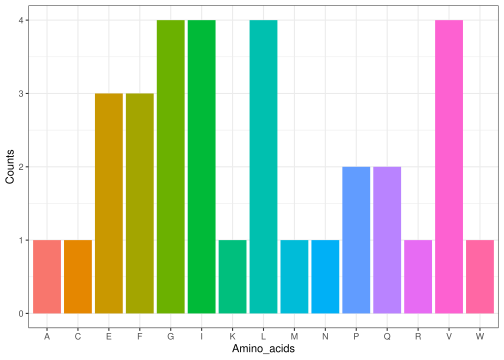
\includegraphics{README_files/figure-latex/unnamed-chunk-6-1.pdf}

\subsection{Discussion}\label{discussion}

\end{document}
